\chapter{Introduction and Background}

The focus on reduction of greenhouse emissions from fossil fuels is today as important as ever. The rapid ongoing modifications of climate conditions are raising concerns and awareness in this regard. Total anthropogenic greenhouse emissions have continued to increase over 1970 to 2010, with larger absolute  increase per decade toward the end of this period, with CO\textsubscript{2} emissions from fossil fuel combustion and industrial processes contributing about 78 \% of the total. Annual anthropogenic GHG emissions have increased by 10 Gtons equivalent of CO2 between 2000 and 2010, with this increase directly coming from energy supply (47 \%), industry (30 \%), transport (11 \%) and buildings (3 \%) sectors \cite{IPCC2014}.

Global warming causes adverse effect and mutations in natural habitats and natural equilibriums of Earth, and is held responsible for increase of atmospheric temperature, acidification of oceans, melting of the permafrost, increased frequency of extreme weather events and others. As a result, many species struggle to adapt to these new environmental conditions and some are facing extinction. Also human related activities are in danger, as the natural habitat become more and more hostile to plants and animals. In the following sections this phenomenon will be explained in more details, and  the role of transportation sector will be highlighted.

\section{Global warming and role of transport section emissions} \label{sec:global_warming}

Global warming and climate change are terms used for describing the increase in surface and ocean temperature registered in the last century. Due to the effect of greenhouse gases, additional energy is stored in the atmosphere and the oceans, causing ice melting and warming of continents and atmosphere. 

\begin{figure}[h]
  \centering
  \includegraphics[width=0.8\textwidth]{figures/introduction/temp_rise.pdf}
  \caption{Temperature rise \cite{GISS2016}}
  \label{antropogenic_ghg_emissions}
\end{figure}

Without additional efforts to reduce GHG emissions beyond those in place today, emissions growth is expected to persist driven by growth in global population and economic activities. Baseline scenarios, those without additional mitigation, result in global mean surface temperature increases in 2100 from \SI{3.7}{\celsius}  to \SI{4.8}{\celsius}  compared to pre-industrial levels \cite{IPCC2014}. Of the 49 Gt CO\textsubscript{2,eq} emitted in 2010, the transportation sector is responsible for 14.3 \% of the total, ranking as the fourth major emitter economic sector after Electricity and Heat production, Agriculture and Land use, and Industry.

\begin{figure}[h]
  \centering
\includegraphics[width=0.8\textwidth]{figures/introduction/antropogenic_ghg_emissions.pdf}
  \caption{Antropogenic GHG emissions by group of gases (1970 - 2010) \cite{IPCC2014}}
  \label{antropogenic_ghg_emissions}
\end{figure}

The scientific community mainly agrees on trying to keep the temperature increase with respect to pre-industrial levels under \SI{2}{\celsius}, that is atmospheric concentrations in 2100 of about 450 ppm CO\textsubscript{2,eq}. The aforementioned scenarios include substantial cuts in anthropogenic GHG emissions by mid century through large scale changes in energy systems and potentially land use. Scenarios reaching these concentrations by 2100 are characterized by lower global GHG emissions in 2050 than in 2010, 40 \% to 70 \% lower globally, and emissions levels near zero Gt CO\textsubscript{2,eq} or below in 2100 \cite{IPCC2014}. In Figure \ref{fig:mitigationscenarios}, the reduction in emissions for the major economic sectors is reported. It's possible to notice how, especially in the case without heavy implementation of carbon dioxide capture plants, the amount of greenhouse gases released in the atmosphere by transport must be greatly reduced.

\begin{figure}[ht]
  \centering
  \includegraphics[width=0.8\textwidth]{figures/introduction/mitigation_scenarios.pdf}
  \caption{Review of different mitigation scenarios for 450 ppm \label{fig:mitigationscenarios}}
\end{figure}

The chart represents a review of the major models and scenarios available to date, and taken into consideration in \cite{IPCC2014}. According to the same study, efficiency enhancements and behavioural changes, in order to reduce energy demand compared to baseline scenarios without compromising development, are a key mitigation strategy in scenarios reaching atmospheric CO\textsubscript{2,eq} concentrations of about 450 to about 500 ppm by 2100.

The transport sector accounted for 27 \% of final energy use and 6.7 Gt CO\textsubscript{2} direct emissions in 2010, with baseline CO\textsubscript{2} emissions projected to approximately double by 2050. Technical and behavioural mitigation measures for all transport modes, plus new infrastructure and urban redevelopment investments, could reduce final energy demand in 2050 by around 40 \% below the baseline \cite{IPCC2014}.

A study by Unger and al. \cite{Unger2010} attributes a radiative forcing value to different economic sectors that are the main emitters in today economy. The radiative forcing concept has been developed in order to quantify the human and natural influence on the climate system, and is defined as the net energy flux difference at the top of the atmosphere. In Figure~\ref{fig:radiative_forcing}, the positive and negative contributions of the different economic sectors are presented. It's important to notice how on-road transportation is foreseen to be the major responsible for increasing of atmospheric energy content in 2020, and the second most important factor in 2100. This is due to the peculiar composition of exhaust gases produced by vehicles: they produce mainly components that contribute to trapping heat while other sectors, as the power sector, produce much more components that trap heat, but the net contribution is reduced by the amount of components as black-carbon, that reflects the solar radiation and contribute to cooling down the atmosphere. 

\begin{figure}[ht]
  \centering
  \includegraphics[width=\textwidth]{figures/introduction/radiative_forcing.png}
  \caption{Radiative forcing due to 2000 level emissions grouped by sector in a) 2020 and b) 2100 \label{fig:radiative_forcing}}
\end{figure}

\section{Current transportation scenario}

The average efficiency of modern internal combustion engines is measured to be around 34 \% - 36 \% for Diesel engines, and around 29 \% - 32 \% for Gasoline engines.

According to the evidence reported in section~\ref{sec:global_warming}, being the transportation sector one of the main culprits for global warming, an increase of the efficiency of passenger vehicles can play an important role in mitigating climate change. Figure~\ref{fig:average_fuel_efficiency} shows how, in the 1980 - 2014 considered timeframe, the specific fuel consumption of U.S. vehicles has been reduced due to technical advancements~\cite{BureauofTransportationStatistics2016}.

\begin{figure}[ht]
  \centering
  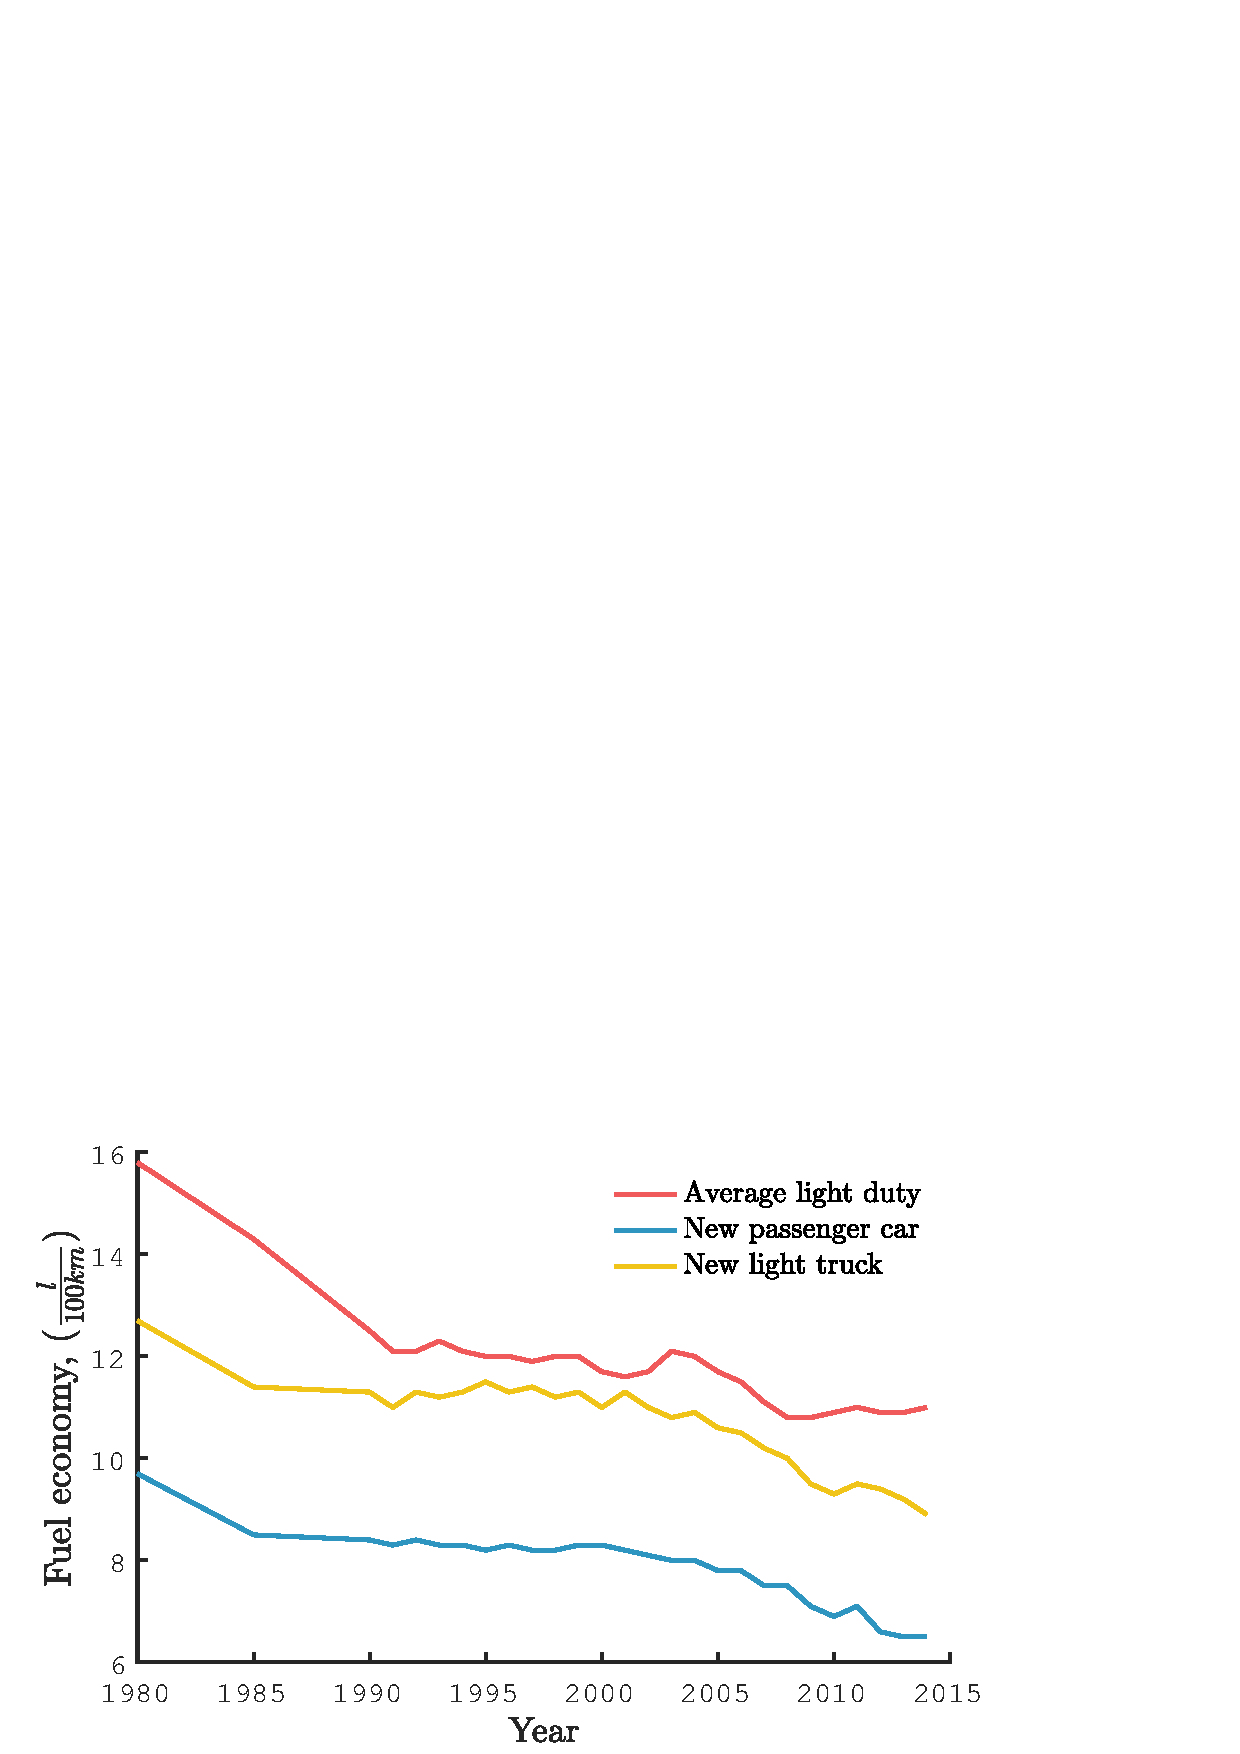
\includegraphics[width=0.8\textwidth]{figures/introduction/average_fuel_efficiency.png}
  \caption{\label{fig:average_fuel_efficiency} }
\end{figure}

Taking a more in depth look at the emissions figure of the transportation economy itself, when considering the energy use by transportation mode in 2013, Highwway is by far the sector that consumes the greater share of the total (83.2 \%), followed by Air transportation (6.9 \%) and Water transportation (3.9 \%). The Highway energy usage can be once again split between Light-duty (52.2 \%), Combination Truck (15.3 \%), Single-unit truck (7.6 \%), and Bus (1.1 \%). Certified air carriers experienced the largest total decrease in fuel consumption, consuming about 3.6 billion fewer gallons of jet fuel in 2014 than in 2000. General aviation gasoline showed the largest percent decrease in fuel consumption from 2000 to 2014, declining by 40.8 percent. Additionally, water modes powered by residual fuel oil also showed a large decrease, declining by nearly 2.6 billion gallons during the same period. Consistent with increases in vehicle-miles traveled, light-duty highway vehicles used about 430 million more gallons of gasoline in 2014 than in 2000~\cite{BureauofTransportationStatistics2016a}.

According to the evidence shown, the amount of effort spent on researching and experimenting new and more advanced means of reducing them is justified. Numerous different strategies are nowadays gaining traction in the automotive field, such as downsizing and turbocharging of gasoline engines, or the use of different cycles, and a more in depth analysis will be provided in Section~\ref{sec:technology_improvements}.

\section{Objectives and structure of the thesis}

The main objective of this thesis is to compare three different technologies that aim at recovering waste heat produced by the internal combustion engine. In particular, these are two different Organic Rankine bottoming cycles paired with an Otto-cycle engine, and a split-cycle engine with isothermal compression and integrated waste heat recovery.

The comparison will be carried out via Matlab/Simulink simulations. A backward-looking model will take as input the velocity profile of a driving cycle for which experimental data is available, then the torque and angular speed at the engine will be calculated through a simulated transmission. Furthermore, engine maps will be extracted from experimental data along with characteristics and performances of the heat exchangers, making possible the calculation of flow rate, temperature and heat flux for both the exhaust gases and the coolant. Once the waste heat data will be available, the bottoming cycle model will be introduced. Starting from the output of the powertrain model, the recovered energy and produced power will be calculated.

\emph{TO BE CONTINUED WITH STRUCTURE}

\chapter{Review of the state of the art}

\section{Evolution in internal combustion engines technology and efficiency}
$\frac{HP}{Displacement}$
In this section a review of the key technical improvements occurred to internal combustion engines in the last decades is presented, among with a brief explanation of the current emission limitation rules for both the USA and Europe. The final section will cover the importance of waste heat recovery and why it needs to be researched and adopted in the next years to achieve the planned emissions limitation objectives.

\subsection{Improvements on overall engine efficiency in the last decades}

Since the petroleum crysis of the '70s, an increasing effort on reduction of fuel consumption and increase of power density has begun.

\begin{figure}[ht]
  \centering
  \includegraphics[width=\textwidth]{figures/review/adj_fuel_economy.pdf}
  \caption{Adjusted CO\textsubscript{2} and fuel economy for vehicles model year from 1975 to 2016\label{fig:adj_fuel_economy} }
\end{figure}

As shown in Figure~\ref{fig:adj_fuel_economy}~\cite{EPA2016}, during the last four decades, the fuel consumption and carbon dioxide emissions has been vastly reduced. This great improvement has been possible thanks to some key technical turning points.

One of the main design aspects that have changed significantly over time is how the fuel is delivered into the engine. Until the early 1980s the majority of engines used carburetors to meter fuel delivered to the combustion chamber. More recently, engines with gasoline direct injection (GDI) have begun to replace engines with port fuel injection. GDI equipped engines were first introduced with very limited production in Model Year (MY) 2007. Eight years later GDI engines were installed in about 42 \% of MY 2015 vehicles, and are projected to achieve a 49 \% market share in MY 2016~\cite{EPA2016}.

Another key aspect of engine design that has been vastly improved is the valve-train. The number of valves per cylinder and the ability to alter valve timing during the combustion cycle allowed significant power and efficiency improvements, and nowadays almost the entire fleet of the most relevant car manufacturers has converted to multi-valve design. While some three and five valve engines have been produced, the vast majority of multi-valve engines are based on 4 valves per cylinder~\cite{EPA2016}. In addition to the number of valves per cylinder, designs have evolved that allow engine valves to vary the timing when they are opened or closed with respect to the combustion cycle, creating more flexibility to control engine efficiency, power, and emissions. In Figure~\ref{fig:improvement_valve_fuel_delivery}, the fuel consumption reduction made possible by the improved valve-train and fuel delivery is shown. 

\begin{figure}[ht]
  \centering
  \includegraphics[width=0.6\textwidth]{figures/review/improvement_valve_fuel_delivery.pdf}
  \caption{Trends of fuel consumption variation with the introduction of major fuel delivery and valve-train control technologies \label{fig:improvement_valve_fuel_delivery} }
\end{figure}

As a result of the new fuel delivery systems, along with other reasons, two very noticeable trends in horsepower and displacement delineated. Average horsepower climbed consistently from MY 1982 to MY 2008. Since MY 2008, horsepower trends have been less consistent, and may be beginning to flatten out. From MY 1975 to 1987, the average engine displacement of new vehicles dropped dramatically by nearly 40 \%. From MY 1988 to 2004, displacement generally grew slowly, but the trend reversed in 2005 and engine displacement has been generally decreasing since. In MY 2016, engine displacement is projected to reach the lowest point on record, below the previous lowest average displacement reached in MY 1987~\cite{EPA2016}.

The contrasting trends in horsepower increase and displacement decrease are a proof of the continued improvements in engine design and of the impact of new technologies. The final result is a steady quasi-linear increase of the power density from around 0.5~$\frac{HP}{Displacement}$ in 1975 to around 1.4~$\frac{HP}{Displacement}$ in 2016, with a growth rate of 0.02~$\frac{HP}{in^{2} \cdot year}$. Also the average number of cylinders has gradually reduced.

In Figure~\ref{fig:technology_trends}, a summary of the time trends of the major innovations is reported.

\begin{figure}[ht]
  \centering  \includegraphics[width=\textwidth]{figures/review/technology_trends.png}
  \caption{Percentage of MY equipped with a certain technology  \label{fig:technology_trends} }
\end{figure}


\subsection{Emission limitations and trends in nowadays technology improvement}
\label{sec:technology_improvements}

Emission limitations are among the main drivers that fostered the continuous strive of greater efficiency in internal combustion engines. In Figure~\ref{fig:emission_standards} a review of the most important emissions standards from across the world, and their Euro equivalence is presented~\cite{Miller2014}. In Figure~\ref{fig:emission_levels} are reported the emission limits for gasoline and diesel powered light vehicles in both the USA and Europe~\cite{Transportpolicy.net2016}.

\begin{figure}[ht]
  \centering
  \includegraphics[width=\textwidth]{figures/review/emission_standards.png}
  \caption{Comparison of emissions standards with reference to Euro standards\label{fig:emission_standards} }
\end{figure}

\begin{figure}[ht]
  \centering
  \includegraphics[width=\textwidth]{figures/review/emissions_levels.png}
  \caption{Emissions limits for a) Gasoline and b) Diesel light vehicles in USA and Europe\label{fig:emission_levels} }
\end{figure}

In order to respect the emission standards imposed by current and future rules, the major car manufacturers are adopting some new technologies and some trends are delineating.



\subsection{The importance of waste heat recovery}




%%% Local Variables:
%%% mode: latex
%%% TeX-engine: xetex
%%% TeX-master: "thesis"
%%% End:
%%% \end{document}
